\section{Экономический раздел}
\label{sec:economy}

\subsection{Планирование разработки системы}

Основой данной выпускной квалификационной работы является <<Разработка системы для поиска и возврата утерянных вещей>>. В данном разделе определяются уровень сложности и затраты на создание программного и аппаратного обеспечения, а также оценивается экономическая выгода, которую можно получить от использования разрабатываемого программного обеспечения.

\subsubsection{Определение трудоемкости и продолжительности работ по созданию УСПД}

В этом разделе определяются уровень сложности и затраты на создание программного и аппаратного обеспечения, а также проводится оценка экономической выгоды от использования разрабатываемого ПО. Процесс разработки включает анализ предметной области, имитационный анализ, создание, настройку и тестирование системы.

\begin{itemize}	
	\item Техническое задание. Регламентированы следующие этапы исследования: составление технического задания, включающего формулировку задач, подбор литературы, сбор исходных данных, определение системных требований, а также определение этапов, фаз и сроков разработки программного обеспечения.
	
	\item Эскизный проект. Этот этап включает в себя использование программных средств для анализа схожих тем, разработки общих программных структур и структур по подсистемам, создания прототипов и документации.
	
	\item Технический проект. Этот этап включает в себя определение требований к программному обеспечению и выбор инструментов и использование программных средств.
	
	\item Рабочий проект. Этап включает компоновку и дизайн, программирование, тестирование и отладку ПО, проектирование плат, а также координацию и утверждение работоспособности всей системы.
	
	\item Внедрение. Подразумевает под собой использование на реальной инфраструктуре; анализ полученных данных в результате исследований, благодаря которым можно будет скорректировать техническую документацию.
\end{itemize}

Трудоемкость работ по созданию программного обеспечения носит вероятностный характер, поскольку определяется суммой сложности этапов и видов работ, оцениваемых экспертами в ручные дни, и зависит от многих факторов, которые трудно учесть.

Трудоемкость каждого вида работ определяется по формуле~(\ref{eq:t_i}).
\begin{equation}\label{eq:t_i}
	t_i=\frac{3 \cdot t_{min} + 2 \cdot t_{max}}{5},
\end{equation}
где $t_{min}$~--- минимально возможная трудоемкость выполнения отдельного вида работ; \\
$t_{max}$~--- максимально возможная трудоемкость выполнения отдельного вида
работ.

Различные виды работ имеют свою продолжительность в календарных днях ($T_{i}$), определяясь по формуле~(\ref{eq:T_i}), в днях:
\begin{equation}\label{eq:T_i}
	T_i=\frac{t_{i}}{\text{Ч}_{i}} \cdot K_{\text{вых}},
\end{equation}
где $t_{i}$~--- трудоемкость работ, человеко-дней; \\
$\text{Ч}_{i}$~--- численность исполнителей, человек; \\
$K_{\text{вых}}$~--- коэффициент, учитывающий выходные и праздничные дни, находится по формуле~(\ref{eq:k_vih}):
\begin{equation}\label{eq:k_vih}
	K_{\text{вых}}=\frac{K_{\text{кал}}}{K_{\text{раб}}},
\end{equation}
где $K_{\text{кал}}$~--- календарные дни; \\
$K_{\text{раб}}$~--- рабочие дни; \\
$K_{\text{вых}}$~--- 1,48.

Далее предоставляется перечень разновидностей и стадий рабочей деятельности по разработке ПО, экспертные оценки, а также рассчитываемые переменные их трудоемкости, а также продолжительность каждого вида работ, рассчитанные по формулам~(\ref{eq:t_i}) и~(\ref{eq:T_i}), представлены в таблице~\ref{tab:work_hours}.

\begin{longtable}{ |x{1cm}|x{3cm}|x{1cm}|x{1cm}|x{1cm}|x{3cm}|x{3cm}| } 
	
	\caption{Расчет трудоемкости и продолжительности работ по созданию ПО и аппаратных средств календарных дней}
	\label{tab:work_hours} \\ 
	
	\hline 
	\parbox[t]{2mm}{\multirow{2}{*}{\rotatebox[origin=c]{90}{\bfseries \textnumero{} работы\hspace{5mm}}}} &
	\multicolumn{1}{p{3cm}|}{\multirow{2}{*}{\parbox{3cm}{\bfseries Стадии разработки}}} & 
	\multicolumn{3}{p{3cm}|}{\bfseries Трудоемкость, чел. дни} & 
	\multicolumn{1}{p{3cm}|}{\bfseries Количество работников, чел.} & 
	\multicolumn{1}{p{3cm}|}{\bfseries Про\-дол\-жи\-тель- ность работ, календарные дни}
	
	\endfirsthead
	
	
	\multicolumn{7}{l}{{Продолжение таблицы \thetable{}.}} \\ \hline
	\parbox[t]{2mm}{\multirow{2}{*}{\rotatebox[origin=c]{90}{\bfseries \textnumero{} работы\hspace{5mm}}}} &
	\multicolumn{1}{p{3cm}|}{\multirow{2}{*}{\parbox{3cm}{\bfseries Стадии разработки}}} & 
	\multicolumn{3}{p{3cm}|}{\bfseries Трудоемкость, чел. дни} & 
	\multicolumn{1}{p{3cm}|}{\bfseries Количество работников, чел.} & 
	\multicolumn{1}{p{3cm}|}{\bfseries Про\-дол\-жи\-тель- ность работ, календарные дни}
	\endhead
	
	\endfoot
	
	\endlastfoot
	
	\hline
	
	&& $t_{min}$ & $t_{max}$ & $t_{i}$ & $\text{Ч}_i$ & $T_i$ \\ \hline
	
	\multicolumn{7}{|c|}{Техническое задание} \\ \hline
	
	1 & - постановка задачи & 3 & 6 & 4.2 & 1 & 6.2 \\ \hline
	
	2 & - подбор литературы & 2 & 3 & 2.4 & 1 & 3.6 \\ \hline
	
	3 & - сбор исходных данных & 4 & 5 & 4.4 & 1 & 6.5 \\ \hline
	
	4 & - определение требований к системе & 3 & 4 & 3.4 & 1 & 5.0 \\ \hline
	
	5 & - определение стадий, этапов и сроков разработки ПО & 2 & 3 & 2.4 & 1 & 3.6 \\ \hline
	
	\multicolumn{7}{|c|}{Эскизный проект} \\ \hline
	
	6 & - анализ программных средств схожей тематики & 7 & 8 & 7.4 & 1 & 11.0 \\ \hline
	
	7 & - разработка общей структуры ПО & 4 & 8 & 5.6 & 1 & 8.3 \\ \hline
	
	8 & - разработка структуры программы и подсистем & 5 & 8 & 6.2 & 1 & 9.2 \\ \hline
	
	9 & - создание прототипа & 4 & 6 & 4.8 & 1 & 7.1 \\ \hline
	
	10 & - документирование & 2 & 3 & 2.4 & 1 & 3.6 \\ \hline
	
	11 & - определение требований к ПО & 3 & 4 & 3.4 & 1 & 5.0 \\ \hline
	
	12 & - выбор инструментальных средств & 3 & 4 & 3.4 & 1 & 5.0 \\ \hline
	
	\multicolumn{7}{|c|}{Рабочий проект} \\ \hline
	
	13 & - программирование & 20 & 25 & 22 & 1 & 32.6 \\ \hline
	
	14 & - тестирование и отладка ПО & 7 & 8 & 7.4 & 1 & 11.0 \\ \hline
	
	15 & - разработка программной документации & 4 & 6 & 4.8 & 1 & 7.1 \\ \hline
	
	16 & - согласование и утверждение работоспособности системы & 2 & 3 & 2.4 & 1 & 3.6 \\ \hline
	
	\multicolumn{7}{|c|}{Внедрение} \\ \hline
	
	17 & - опытная эксплуатация & 6 & 8 & 6.8 & 1 & 10.1 \\ \hline
	
	18 & - анализ данных, полученных в результате эксплуатации & 2 & 4 & 2.8 & 1 & 4.1 \\ \hline
	
	19 & - корректировка технической документации по результатам испытаний & 1 & 2 & 1.4 & 1 & 2.1 \\ \hline
	
	& {\bfseries Общая трудоемкость разработки} &&& 98 && 144 \\ \hline
\end{longtable}

Следовательно, общая продолжительность проведения работ $T_{i} = 144$.

\subsubsection{Построение ленточного графика проведения исследования}

В качестве инструмента планирования используется ленточный график~(\ref{fig:work_waterfall}).
\begin{figure}[H]
	\centering
	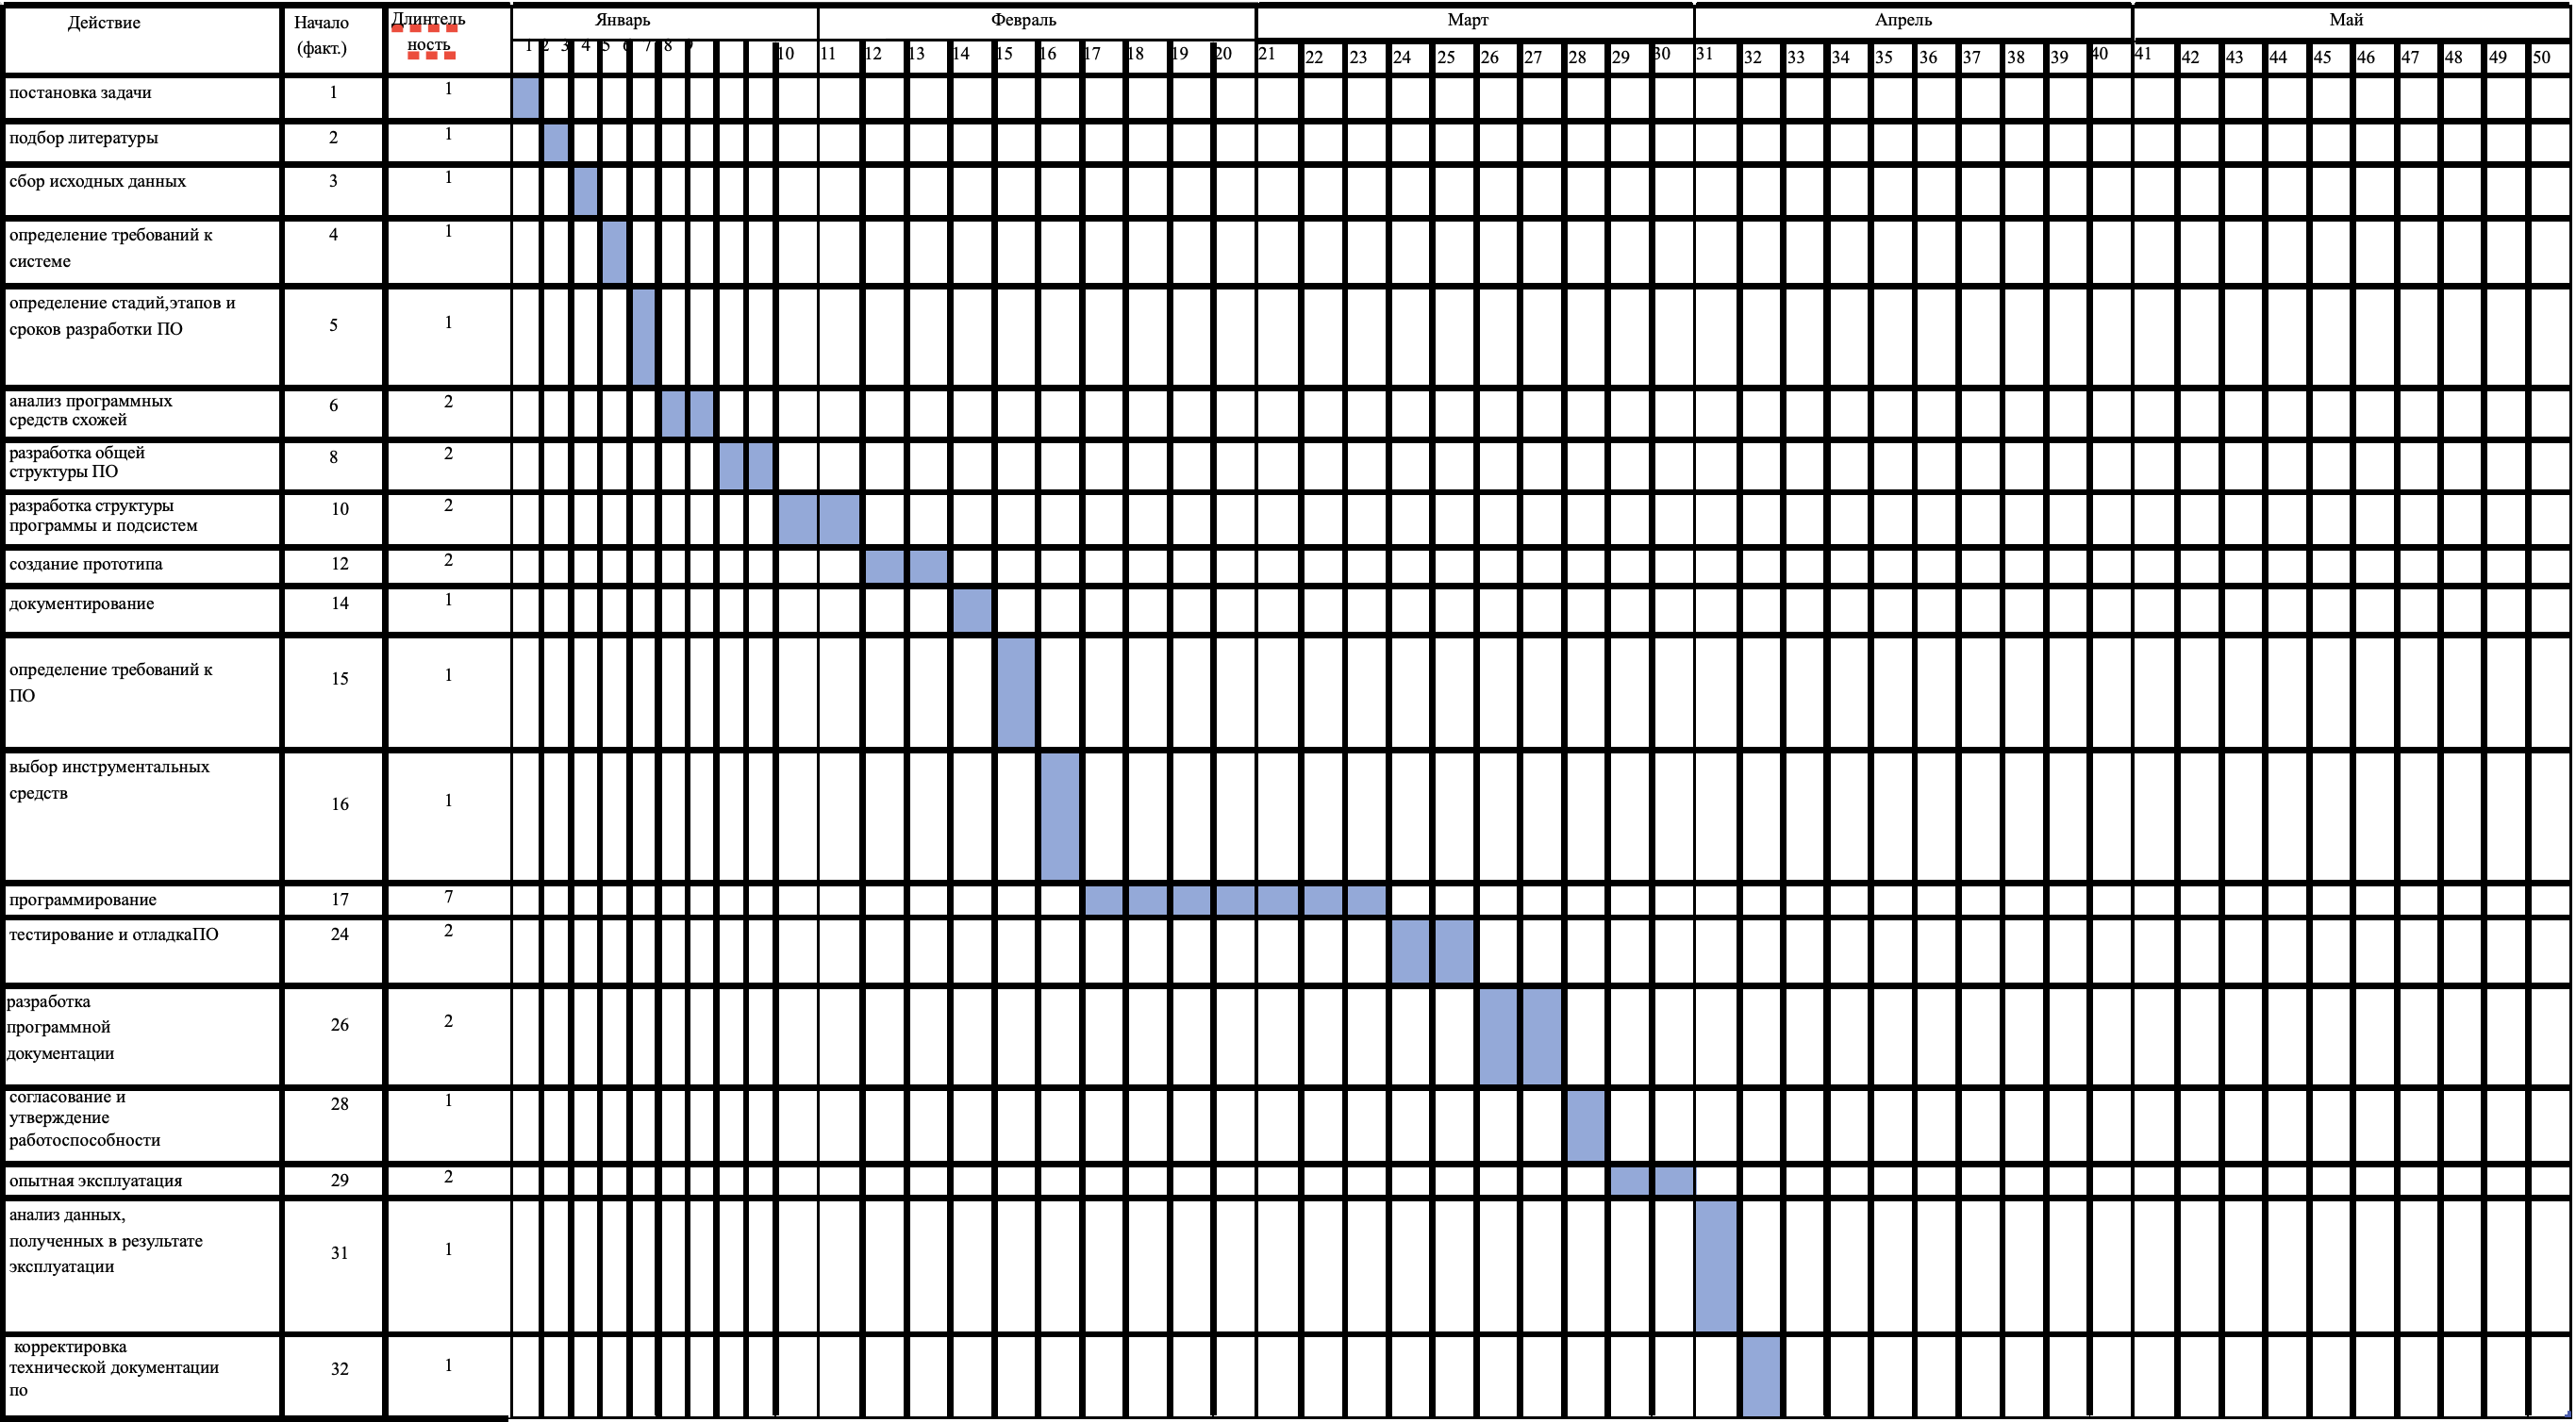
\includegraphics[width=.7\textheight,angle=90,origin=c]{images/work_waterfall}
	\parskip=6pt
	\caption{Ленточный график}
	\label{fig:work_waterfall}
\end{figure}

Подобный график позволяет наглядно представить логическую
последовательность и взаимосвязь отдельных работ. График представляет собой
таблицу с перечислением названий стадий разработки, видов работ, длительность выполнения работ. Данный график построен по данным таблицы~\ref{tab:work_hours}. В этом графике временная единица выполнения работ оценивается в 3 дня.

\subsection{Расчет сметы затрат на разработку представленной работы}

Сметная стоимость проектирования и внедрения программы включает в себя затраты, определяемые по формуле~(\ref{eq:estimate}):
\begin{equation}\label{eq:estimate}
	C_{\text{пр}} = C_{\text{осн}} + C_{\text{доп}} + C_{\text{соц}} + C_{\text{м}} + C_{\text{маш.вр}} + C_{\text{н}},
\end{equation}
где $C_{\text{пр}}$~--- стоимость разработки ПО; \\
$C_{\text{осн}}$~--- основная заработная плата исполнителей; \\
$C_{\text{доп}}$~--- дополнительная заработная плата исполнителей, учитывающая потери времени на отпуска и болезни (принимается в среднем 10\% от основной заработной платы; \\
$C_{\text{соц}}$~--- отчисления в фонд социального страхования – 30\% от основной и дополнительной заработной платы; \\
$C_{\text{м}}$~--- затраты на используемые материалы; \\
$C_{\text{маш.вр}}$~--- стоимость машинного времени; \\
$C_{\text{н}}$~--- накладные расходы включают затраты на управление, уборку, ремонт, электроэнергию, отопление и др. (принимаются в размере 60\% от основной и дополнительной заработной платы).

\subsubsection{Основная заработная плата исполнителей}

На статью «Заработная плата» относят заработную плату научных, инженерно-технических и других работников, непосредственно участвующих в разработке ПО. Расчет ведется по формуле (\ref{eq:salary}):

\begin{equation}\label{eq:salary}
	\text{З}_{\text{исп}} = \text{З}_{\text{ср}} \cdot T,
\end{equation}
где $\text{З}_{\text{исп}}$~--- заработная плата исполнителей (руб.); \\
$\text{З}_{\text{ср}}$~--- средняя тарифная ставка работника организации разработчика ПО (руб./чел./дни); \\
$T$~--- трудоемкость разработки ПО (чел.дни).

$\text{З}_{\text{ср}}$ определяется по формуле~(\ref{eq:work_tariff}):
\begin{equation}\label{eq:work_tariff}
	\text{З}_{\text{ср}} = \frac{C}{\text{Ф}_{\text{мес}}},
\end{equation}
где $C$~--- зарплата труда на текущий момент времени (руб./мес.); \\
$\text{Ф}_{\text{мес}}$~--- месячный фонд рабочего времени исполнителя (дни).

Затраты на статью <<Заработной платы>> приведены в таблице~\ref{tab:salary}.
\begin{table}[htb]
	\caption{Затраты на заработную плату}
	\centering
	
	\tolerance=0
	\emergencystretch=10pt
	\hyphenpenalty=0
	\exhyphenpenalty=0
	\begin{tabular}{ |x{1cm}|x{2cm}|x{2cm}|x{2cm}|x{3cm}|x{2cm}| } 
		\hline
		\textnumero{} & Исполнитель & Оклад, руб./мес. & Оклад, руб./мес. & Трудоемкость, чел.дни & Сумма, руб. \\ \hline
		
		1 & Инженер-программист & 70000 & 3500 & 98 & 343000 \\ \hline
		
		\multicolumn{4}{|x{7cm}|}{Общая основная заработная плата исполнителей, $C_{\text{осн}}$} & 98 & 343000 \\ \hline
		
	\end{tabular}
	\label{tab:salary}
\end{table}

\subsubsection{Дополнительная заработная плата исполнителей}

Дополнительная заработная плата на период разработки ПО рассчитывается относительно основной и составляет 10\% от её величины, рассчитывается по формуле~\ref{eq:addit_salary}.
\begin{equation}\label{eq:addit_salary}
	C_{\text{доп}} = C_{\text{осн}} \cdot 0{,}1 = 34300\,\text{(руб. )}.
\end{equation}

\subsubsection{Расчет отчислений на социальное страхование}

Отчисления на социальное страхование рассчитываются относительно выплаченной заработной платы по формуле~(\ref{eq:social_pay}). Составляют 30%:
\begin{equation}\label{eq:social_pay}
	\begin{array}{l}
		C_{\text{соц}} = ( C_{\text{доп}} + C_{\text{доп}} ) \cdot 0{,}3 \\ 
		C_{\text{соц}} = (34300 + 343000) \cdot 0{,}3 = 113190\,\text{(руб. )}
	\end{array}
\end{equation}

На эту статью относят все затраты на магнитные носители данных, бумагу, для печатных устройств, канцтовары и др. Затраты по ним определяются по экспертным оценкам. Расчет расходов на материалы приведен в таблице~\ref{tab:additional_pay}.

\begin{table}[htb]
	\caption{Расчёт расходов на материалы}
	\centering
	
	\tolerance=0
	\emergencystretch=10pt
	\hyphenpenalty=0
	\exhyphenpenalty=0
	\begin{tabular}{ |x{1cm}|x{4cm}|x{4cm}|x{4cm}| } 
		\hline
		\textnumero{} & Материалы & Количество, штуки & Стоимость, рубли \\ \hline
		
		1 & Бумага писчая, листов & 1000 & 800 \\ \hline
		
		2 & Картридж для принтера, шт. & 1 & 1000 \\ \hline
		
		3 & Другие канцтовары & - & 1000 \\ \hline
		
		\multicolumn{3}{|x{12cm}|}{Общая стоимость материалов, $C_{м}$} & 2800 \\ \hline
		
	\end{tabular}
	\label{tab:additional_pay}
\end{table}

\subsubsection{Накладные расходы}

На статью «Накладные расходы» относят расходы, связанные с управлением и организацией работ. Накладные расходы рассчитываются относительно основной заработной платы. Величина накладных расходов принимается равной 60~\% от основной зарплаты исполнителей. Формула расчета~(\ref{eq:overheads}):
\begin{equation}\label{eq:overheads}
	C_{\text{н}} = C_{\text{осн}} \cdot K,
\end{equation}
где $C_{\text{н}}$~--- накладные расходы; \\
$C_{\text{осн}}$~--- основная заработная плата исполнителей; \\
$K$~--- коэффициент учета накладных расходов.

\begin{equation*}
	C_{\text{н}} = 343000 \cdot 0{,}6 = 205800\,\text{(руб.)}
\end{equation*}

\subsubsection{Расчет стоимости машинного времени}

Затраты на машинное время, необходимое для разработки ПО, расходы на приобретение и подготовку материалов научно-технической информации, расходы на использование средствами связи. Расчет затрат на машинное время осуществляется по формуле~(\ref{eq:machine_pay}):

\begin{equation}\label{eq:machine_pay}
	C_{\text{маш.вр}} = K_{\text{маш.вр}} \cdot \text{З}_{\text{маш.вр}}
\end{equation}
где $К_{\text{маш.вр}}$~--- тарифная стоимость одного часа машинного времени ($К_{\text{маш.вр}} = 60~\text{(руб./час)}$); \\
$\text{З}_{\text{маш.вр}}$~--- машинное время, используемое на проведение работ.

Необходимое количество машинного времени для реализации проекта по разработке программы рассчитывается по формуле (\ref{eq:machine_time}):
\begin{equation}\label{eq:machine_time}
	\text{З}_{\text{маш.вр}} = t_i \cdot T_{\text{см}} \cdot T_{\text{ср.маш}},
\end{equation}
где $t_i$~--- трудоемкость работ, чел.дней; \\
$T_{\text{см}}$~--- продолжительность рабочей смены (При пятидневной рабочей неделе $T_{\text{см}} = 8 \text{ч.}$); \\
$T_{\text{ср.маш}}$~--- средний коэффициент использования машинного времени ($T_{\text{ср.маш}} = 0{,}7$).

Из этого следует:
\begin{equation*}
	\text{З}_{\text{маш.вр}} = 98 \cdot 8 \cdot 0{,}7 = 548{,}8\,(\text{ч.})
\end{equation*}

Стоимость машинного времени составит:
\begin{equation*}
	C_{\text{маш.вр}} = 60 \cdot 548{,}8 = 32928\,(\text{руб.})
\end{equation*}

Результаты расчета затрат на проектирование программного обеспечения
сведены в таблице~\ref{tab:project_arch}.

\begin{table}[htb]
	\caption{Расчёт расходов на материалы}
	\centering
	
	\tolerance=0
	\emergencystretch=10pt
	\hyphenpenalty=0
	\exhyphenpenalty=0
	\begin{tabular}{ |x{1cm}|x{3.5cm}|x{3.5cm}|x{3.5cm}|x{1cm}| } 
		\hline
		\textnumero{} & Наименование статей & Обозначение & Сумма, руб. & В \% к итогу \\ \hline
		
		1 & Основная заработная плата & $C_{\text{осн.}}$ & 343000 & $46{,}86$ \\ \hline
		
		2 & Дополнительная заработная плата & $C_{\text{доп.}}$ & 34300 & $4{,}69$ \\ \hline
		
		3 & Отчисления на социальные нужды & $C_{\text{соц.}}$ & 113190 & $15{,}46$ \\ \hline
		
		4 & Материалы & $C_{\text{м.}}$ & 2800 & $0{,}38$ \\ \hline
		
		5 & Стоимость машинного времени & $C_{\text{маш.вр.}}$ & 32928 & $4{,}5$ \\ \hline
		
		6 & Накладные расходы & $C_{\text{н.}}$ & 205800 & $28{,}11$ \\ \hline
		
		\multicolumn{2}{|x{4.5cm}|}{Итого:} & $C_{\text{осн.}}$ & 732018 & 100 \\ \hline
		
	\end{tabular}
	\label{tab:project_arch}
\end{table}

Следовательно, себестоимость разработки составляет 732018 руб.

Данная программа может быть реализована на рынке. При расчетном количестве реализованных программ ($n = 5$) оптовая цена программы ($\text{Ц}_{\text{опт}}$) может быть рассчитана по формуле~(\ref{eq:opt_price}):
\begin{equation}\label{eq:opt_price}
	\text{Ц}_{\text{опт}} = \frac{C_{\text{пр}}}{n} + \text{П}
\end{equation}
где $C_{\text{пр}}$~--- себестоимость разработки программы; \\
$\text{П}$~--- прибыль, определяется по формуле~(\ref{eq:profit}):
\begin{equation}\label{eq:profit}
	\text{П}_{i} = \text{У}_{\text{р}} \cdot \frac{C_{\text{пр}}}{n} \cdot 100
\end{equation}
где $\text{У}_{\text{р}}$~--- средний уровень рентабельность ($\text{У}_{\text{р}} = 20\%$).

Таким образом, оптовая цена программы составит:
\begin{equation*}
	\text{Ц}_{\text{опт}} = \frac{732018}{5} + \left( \frac{732018}{5} \cdot 0{,}2 \right) = 146403{,}6 + 29280{,}72 = 175684{,}32 \,(\text{р.})
\end{equation*}

Отпускная цена реализации программы потребителям ($\text{Ц}_{\text{опт}}$), рассчитывается по формуле:
\begin{equation*}
	\text{Ц}_{\text{опт}} = \text{Ц}_{\text{опт}} + \text{НДС}
\end{equation*}
где $\text{НДС}$~--- налог на добавленную стоимость, рассчитывается в соответствии с действующей ставкой этого налога~--- 20\% от оптовой цены программы.

\begin{equation*}
	\text{Ц}_{\text{опт}} = 175684{,}32 + (175684{,}32 \cdot 0{,}2) = 210821{,}18 \,(\text{руб.})
\end{equation*}

Следовательно, отпускная цена программы составит $175684{,}32$ руб., в том числе НДС~--- $35136{,}86$ руб.